
%This section describes the early childhood treatments experienced by the cohorts in our study. We compare state, religious, and municipal systems, considering similarities and differences in administration and programming. To better understand the evolution of various early childhood options apart from what was available in the literature, we administered a historical survey in Reggio Emilia, Parma, and Padova to quantify pedagogical and administrative features of other available childcare experiences available from 1950-2010 \citep{CEHD_2016_Historical-Analysis}. We also sourced data from municipal archives of Reggio Emilia, Parma, and Padova to document child enrollment and teacher staffing of local preschools; we successfully gathered historical materials from the municipal offices of Reggio Emilia and Padova, and from Reggio Children \citep{Padova-Admin-Data_1964-2011,Reggio-Admin-data_1966-2006,Reggio-Annual-Journals_1994-2011}. Based on our new knowledge of similarities and differences across early childhood systems, we document our expectations for variance in outcomes between the Reggio Approach and alternative treatments.  

\subsection{The Reggio Approach}

Of the three municipal systems we compare, Reggio Emilia is particularly notable for its significant investment in innovative municipal programs and services. It is the earliest municipal system to evolve, and historically offers the largest number of municipal infant-toddler and preschool sites.\footnote{Similar to Parma and Padova, Reggio Emilia contracts with local private providers and cooperatives to offer a number of infant-toddler and preschool slots according to municipal regulations. These ``affiliated'' programs may not follow the Reggio Approach nor the municipal approaches in Parma and Padova. Accordingly, we do not include those who were enrolled in affiliated programs in our evaluation.} While eligible, Reggio Emilia did not receive state funding for its municipal early childhood system until the 1990s and 2000s. Ironically, the municipality contributed funds to its local state schools each decade from the 1970s. In 1994, Reggio Approach staff provided training for religious preschool teachers in Reggio Emilia. 
%SK: Should we add a cite per Daniela del B ``most  the principles of the Reggio Approach have become increasingly part of a large number of childcare experience in Italy and Europe (you can cite Bennet 2012 and Lazzari and Vandenbroek 2012) from our paper''? I think this perspective is supported by the historical survey. Also not sure whether JJH will want to include one of her citations...

The Reggio Approach is a form of progressive early childhood education influenced by Loris Malaguzzi, an educator promoting the educational practices and psychological theories of Dewey, Piaget, Erikson, Vygotsky, Bronfenbrenner, Kagan, and Gardner. In 1963, Reggio Emilia opened its first preschool for children aged 3-6 years. In 1965, municipal policies were enacted to provide funding for infant-toddler centers for children aged 3 months to 3 years; in 1971, the first site opened. Reggio Emilia's municipal early childhood system thus preceded Italy's key legislative reforms that established state-run preschools and mandated the local provision of infant-toddler centers \citep{Cagliari-etal-eds_2016_BOOK_Loris-Malaguzzi}. The Reggio Approach views curriculum as an ongoing, collaborative project without pre-determined learning goals or timelines. There is no institutionally-prescribed content knowledge that educators convey to children for ``school readiness.'' In contrast, teachers and children are viewed as researchers and co-creators of knowledge. For example, educators, children and families collaborate to define a question or topic. Learning is then pursued following a scientific process: theories are shared, tested, and revised through dialogue. 

In Reggio Approach preschools, the educative team is assigned specialized roles. Each incoming class of approximately twenty-five 3-year-olds is assigned two full-time co-teachers (teacher-child ratio of 2:25); at least 1 of the 2 teachers remains with this cohort of homogeneous-aged children for three consecutive years. This extended time provides continuity of care for children and enables strong teacher-family engagement. Each preschool site is further staffed by a full-time atelierista, an instructor with a background in visual arts. Teachers observe children's development, interact with children through questions and dialogue, and provide scaffolding to support learning. Children demonstrate their emerging knowledge through creative learning activities and art, with aid from the atelierista. Teachers document each child's development in a portfolio---a collection of work---which is shared and discussed with children and parents over the year \citep{Rinaldi_2006_ReggioEmilia_BOOK,Giudici-Nicolosi_2014_Reggio-Approach}. Auxiliary site staff, such as cooks and janitors, are considered members of the educative team and participate in trainings and professional development. A pedagogista---or educative coordinator---with a higher degree in psychology or education is assigned to support professional development on a biweekly basis for the educative staff of approximately 4-5 municipal preschools. 

The Reggio Approach school environment reflects a light-filled, open interior design, furnished with natural materials and a garden. Each site is equipped with an atelier, or dedicated studio laboratory used for creative instructional activities. In-house kitchens are surrounded by glass walls, to include children in the meal process, and is used daily for preparing meals. Reggio Approach preschools and infant-toddler centers are open five full-time days per week from September through June \citep{Giudici-Nicolosi_2014_Reggio-Approach}. Extended day options are available at a majority of Reggio municipal sites throughout the school year, as is educational programming throughout July. Children with disabilities and single parents have been prioritized in admission criteria from the early 1970's \citep{Edwards-etal-eds_1998_Hundred-Languages}. The engagement of families is embedded in Reggio practices, as is the invitation to all community members to participate in school management \citep{CEHD_2016_Historical-Analysis,Cagliari-etal-eds_2016_BOOK_Loris-Malaguzzi}. 



\subsection{State Preschool for Ages 3-6 Years}
In 1968, law 444 mandated the provision and funding of free, public preschools \textit{only} where local demand was not already met by existing non-state systems \citep{Hohnerlein_2009_Paradox-Public-Preschools}.\footnote{In state programs, parents pay only for meals, transportation, and extras such as field trips and extracurricular lessons.}\footnote{The state does not offer infant-toddler childcare but regulates and subsidizes local programs through regional governments.}  Historical records indicate that state preschools first appeared in Reggio Emilia and Padova between 1973-1975 \citep{Padova-Admin-Data_1964-2011,Reggio-Admin-data_1966-2006,Reggio-Annual-Journals_1994-2011}. While the state is currently the largest provider of preschool education in Italy, enrollment in state preschools in Reggio Emilia, Parma, and Padova have historically lagged behind municipal and religious programs.

State preschools are administrated with local primary and middle schools, operating as a single comprehensive institution for children aged 3 up to 17 years. Orientamenti, or national guidelines, provide the framework for state programs. Orientamenti are periodically revised to reflect current educational practices and political ideology.\footnote{For example, religious teaching was originally required by law in all state preschools. Subsequent revisions allowed parents to opt their child out of religious teaching, however, alternative educational experiences were not guaranteed \citep{CEHD_2016_Historical-Analysis}.} 

Reports suggest that Orientamenti were historically influenced by municipal programs in the region of Emilia Romagna, including Reggio Emilia, Milan, and Pistoia \citep{OECD_2001_Italy-Country-Note}. In contrast to municipal programs in Reggio Emilia, Parma and Padova, however, state preschools do not offer extended hours to working families; state teachers work shorter hours than their municipal counterparts and by law receive equivalent pay to teachers in primary schools. Improved Orientamenti, along with revised state policies mandating lower teacher-child ratios and higher qualifications for teacher education, are proposed as key quality indicators associated with diminishing disparities in state and non-state programs by the end of the 20th century \citep{Hohnerlein_2015_Development-and-Diffusion}. Below we list key historical revisions to Orientamenti, documenting mandated quality improvements in state preschools in the years that our cohorts were eligible to enroll.

\begin{itemize}
 \item Revisions to Orientamenti and State Policies 
 \begin{itemize}
 	\item In 1969, Orientamenti focused on education, development and care \citep{Corsaro_1996_Early-Edu,Hohnerlein_2015_Development-and-DiffusionEnrollment}.
	\item In 1991, Orientamenti emphasized social, affective and cognitive development, defining play, mealtime behavior, and collaborative skills as the key tasks of early childhood \citep{Corsaro_1996_Early-Edu}. 
	\item In 1997, revised teacher requirements included university degrees and supervised experience, expanding traditional teacher training from Catholic institutions to secular higher education \citep{Ghedini_2001_Ital-Natl-Policy}. 
	\item In the early 2000's, infant-toddler services were first recognized as educational in nature, for the development of social, emotional, and cognitive skills.\footnote{We highlight the timing in comparison to the evolution of educational approaches offered by municipal infant-toddler programs in Reggio Emilia (by 1971), in Parma (by mid-late 1970s) and in Padova (by 1990) \citep{CEHD_2016_Historical-Analysis}.} 
 \end{itemize}
 \end{itemize}

The table below reflects the evolution of state mandates for minimum teacher-child ratios in the years our 5 cohorts were eligible for preschool. 

\begin{table}
\begin{center}
\caption{Evolution of Teacher-Child Ratios for children aged 3-6 years}
\label{tab:ratios}
\begin{tabular}{c c}
\toprule
Years & \multicolumn{1}{C{7em}}{Teacher-Child Ratio} \\
\midrule
1955-1956 & 1:36.9 \\
1969-1979 & 1:30.3 \\
1971-1972 & 1:27 \\
1980-1981 & 1:17.3 \\
1995-1996 & 1:13 \\
\bottomrule
\end{tabular}
\end{center}
\small
Source: \citet {Hohnerlein_2015_Development-and-Diffusion}
\end{table}

To summarize, the five cohorts in our evaluation had differential access to state preschools in each city, and those who enrolled in state programs experienced varying early childhood curricula and administrative practices. We hypothesize that the degree to which state preschool experiences vary in our sample is wider between age cohorts than between cities, however, we predict that state preschools in Reggio Emilia are more similar to the Reggio Approach than state preschools in Parma and Padova. 

\subsection{Religious Preschool}

The Catholic Church is the oldest non-state early childhood provider in Italy, offering both religious training and charitable social services for disadvantaged children since the 19th century \citep{OECD_2001_Italy-Country-Note}. While the Church does not offer infant-toddler programming nor a cohesive national system of preschool education, local religious programs began to assemble federations in the mid-1970s. Within federations, local religious sites are enabled to offer independent programs. 

The second half of the 20th century, however, marks a downward trend in enrollment and relative quality of religious early childhood programming throughout Italy.\footnote{Prior to 1968, more than 50\% of Italian children were enrolled in childcare provided mainly by the Church \citep{Hohnerlein_2009_Paradox-Public-Preschools}. Between 1981 and 1998, as the number of municipal and state preschools increased in Italy, enrollment in religious preschools dropped to 42.4\%.} Enrollment trends are reportedly associated with policies allowing non-state schools to operate ``without financial burdens on the state''; religious schools were thus perceived for affluent families that could afford the tuition \citep{Ribolzi_2013_Italy,Hohnerlein_2009_Paradox-Public-Preschools}. Enrollment trends in Reggio Emilia, Parma, and Padova reflect national levels. For the oldest four cohorts in our study, tuition for religious preschools in each of the 3 cities was comparatively more expensive than municipal and state programs. 

Equity in public subsidies was mandated in the late 1990s for non-state programs that met state guidelines. Coincidentally, religious programs began significant efforts to improve and quantify program quality \citep{Malizia-Cicatelli_2011_BOOK_Catholic-School}. For example, religious educators were replaced with secular teachers trained in higher institutions and teacher-child ratios began to reflect state standards. Parents of the youngest cohort, born in 2006, who enrolled in equitable religious programs were eligible for subsidized tuition on a sliding-scale basis, and their children experienced educational programming that reflected an influence by municipal systems in Emilia Romagna, including Reggio Emilia \citep{Hohnerlein_2009_Paradox-Public-Preschools,OECD_2001_Italy-Country-Note}. For example, while religious programs historically did not provide infant-toddler education, by the late 1990's, some sites in each of the three cities began to offer transitional programming for children aged 24 months \citep{Malizia-Cicatelli_2011_BOOK_Catholic-School,CEHD_2016_Historical-Analysis}. 

\subsection{Comparison of Early Childhood Systems in Reggio Emilia, Parma, and Padova}

Published literature about the municipal early childhood systems in Parma and Padova is scarce. To better document these programs, we rely on data from the historical survey, reported by local experts in Reggio Emilia (municipal and state only); in Parma (municipal only); and in Padova (municipal, state, and religious).

Results from the historical survey indicate that early childhood education systems within Reggio Emilia, as well as in Parma and Padova, share certain features of program administration, practices for at-risk children and families, and pedagogical methods. The general trend shows that the components endorsed by the Reggio Approach are increasingly present in other systems, albeit in different degrees. We interpret the results from the historical survey as evidence for potential spillovers into alternative treatments; it is widely accepted that Malaguzzi and other Reggio Emilia municipal leaders influenced ongoing state policies and legislation. 

\subsubsection{Overview of Historical Survey} \label{sec:survey-overview}

%NOTE: PLEASE KEEP THE PARAGRAPH BELOW 
Other early childhood education systems within Reggio Emilia, as well as in Parma and Padova, share certain features of program administration, practices for at-risk children and families, and pedagogical methods. To better compare these systems, we administered a historical survey to current and retired school administrators and educative coordinators from each system in each city. Survey responses were received from the following systems that allowed us to document the history of early childhood programming in each municipality: in Reggio Emilia, municipal and state; in Parma, municipal; and in Padova, municipal, state, and religious. Responses were also received from religious systems in Reggio Emilia and in Parma, however, they did not include historical data prior to 2000. 

%\noindent\textbf{[YKK: I think since the tables show what questions were asked, it may be better to move the list of all questions to the appendix and just explain them briefly in the main paper, which I did. What do you think? SK: Noted, and I edited the text somewhat.]}
The historical survey is designed to compare administrative and pedagogical components present in the Reggio Approach with each of the other systems. The survey was developed based on published program descriptions, and confirmed by expert scholars with firsthand knowledge of the Reggio Approach and early childhood programs in northern Italy.\footnote{See \citet{Edwards-etal-eds_1998_Hundred-Languages} and \citet{Corsaro_2008_Policy-Practice}.} The questionnaire includes administrative program operations including staffing, supervision, enrollment, and funding. It also considers pedagogy and educational practices for children's learning in various dimensions. For a more detailed summary of questions, see Appendix \ref{sec:survey}.

\subsubsection{Enrollment in Early Childhood Systems}

Figure \ref{fig:enrollment} explores the similarities and difference in enrollment statistics in each of the three cities \citep{Padova-Admin-Data_1964-2011,Reggio-Admin-data_1966-2006,Reggio-Annual-Journals_1994-2011}. Note that enrollment data is not available for Parma except for the year 2010. 

Historically, Padova demonstrates the highest rate of preschool attendance. We also see that Reggio Emilia and Padova observed increases in preschool enrollment; by the 1990s, almost all eligible children are enrolled in preschool. Trends in municipal preschool enrollment demonstrate an increase during the 1970s and the 1980s in Reggio Emilia and Padova. Historically, in both Reggio Emilia and Padova, state preschool enrollments increased whereas religious preschool enrollment decreased. In Parma, enrollment statistics in 2010 are similar to those of Reggio Emilia. 

\begin{figure}[H]
      \centering
        \begin{subfigure}[t]{0.49\textwidth}
          \includegraphics[width=\textwidth]{../../output/image/enroll_num_graph.eps}       
\caption{Num. of Children Enrolled in Preschool}        
        \end{subfigure}
        \begin{subfigure}[t]{0.49\textwidth}
          \includegraphics[width=\textwidth]{../../output/image/enroll_per_graph.eps}       
 \caption{Percentage of Ages 3-5 Enrolled in Preschool}        
        \end{subfigure}
        \begin{subfigure}[t]{0.49\textwidth}
          \includegraphics[width=\textwidth]{../../output/image/enroll_per_muni_graph.eps} 
        \caption{Percentage of Enrollment in Municipal Preschools}        
        \end{subfigure}
        \begin{subfigure}[t]{0.49\textwidth}
          \includegraphics[width=\textwidth]{../../output/image/enroll_per_stat_graph.eps}
            \caption{Percentage of Enrollment in State Preschools}       
        \end{subfigure}
      \begin{subfigure}[ht]{0.48\textwidth}
        \includegraphics[width=\textwidth]{../../output/image/enroll_per_priv_graph.eps}
        \caption{Percentage of Enrollment in Religious Preschools}
        \label{fig:large}
      \end{subfigure}
      \caption{Enrollment Statistics}  \label{fig:enrollment}
    \end{figure}

\subsubsection{Results of the Historical Survey}

The historical survey demonstrates similarities and differences in administrative and pedagogical components between the Reggio Approach and alternative treatments. In Table \ref{tab:programoperation}, we consider surveyed reports of administrative operations of early childhood system from 1960 through 2010 against systematic features of Reggio Emilia's municipal program. We find that each of the municipalities, state, and religious systems invested in early childhood programming in different times and in different ways. We find innovation in the Reggio Approach and considerable investment by the Reggio Emilia municipality in a large and comprehensive early childhood system as well as in local state and religious preschools. 


To summarize, we present the similarities and differences between the different programs in Figures~\ref{fig:agg-admin} and~\ref{fig:agg-ped}. Using results from the structured interviews, we compute the number of administrative and pedagogical components that each program shares with the Reggio Approach by school type, city, and year. We examine 14 administrative components and 16 pedagogical components (not all of the pedagogical components were present in the Reggio Approach). Over time, many of the programs other than the state programs, adopted more features present in the Reggio Approach. This is especially true of the Parma municipal program when examining administrative components. The other programs did not adopt as many pedagogical components as they did administrative ones. Even though the Reggio Approach remained distinctive when considering the sum of its elements, many of the alternative schools evolved to include certain elements.

\begin{figure}[H]
\begin{center}
\begin{subfigure}[b]{0.49\textwidth}
	\caption{Number of Administrative Characteristics in Common with the Reggio Approach}\label{fig:agg-admin}
	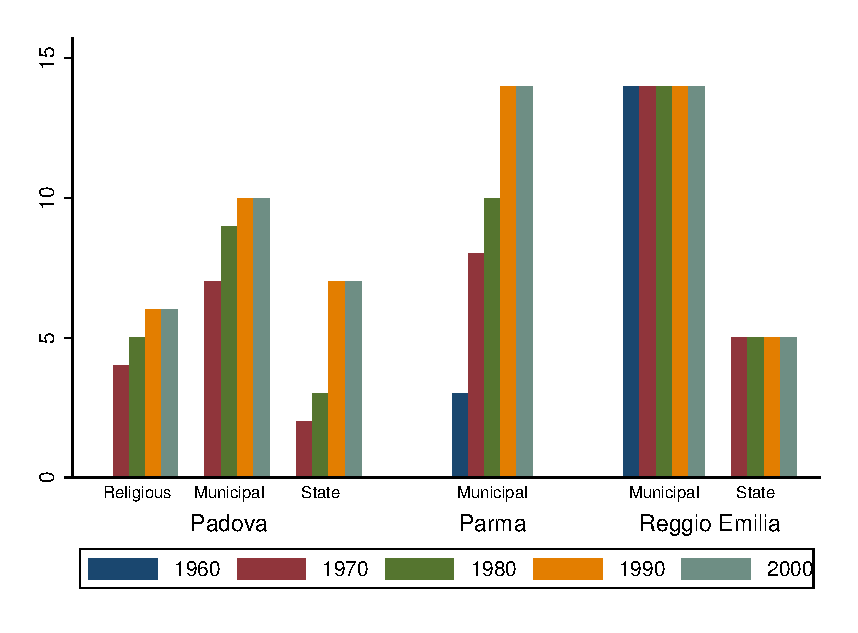
\includegraphics[width=\textwidth]{../../output/aggregateAdministrative.eps}
\end{subfigure}%
~
\begin{subfigure}[b]{0.49\textwidth}
	\caption{Number of Pedagogical Characteristics in Common with the Reggio Approach}\label{fig:agg-ped}
	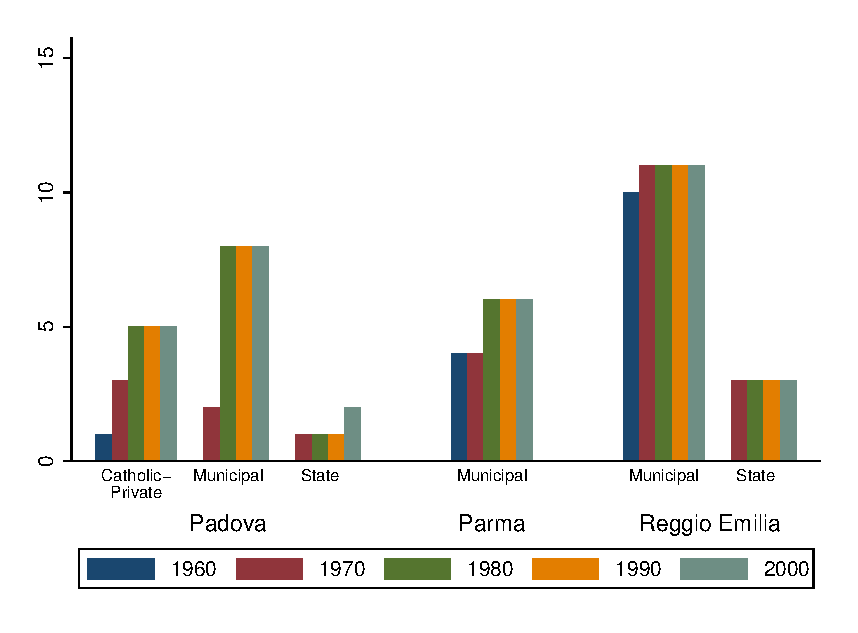
\includegraphics[width=\textwidth]{../../output/aggregatePedagogical.eps}
\end{subfigure}%
\end{center}
\raggedright \footnotesize Note: These graphs show the number of administrative and pedagogical components that each program has in common with the Reggio Approach. We consider 14 administrative components and 16 pedagogical components. Some of the pedagogical components were not present in the Reggio Approach. 
\end{figure}

We emphasize the results of the survey for items that are related to prioritizing disadvantaged children. Municipal schools in the three cities shared priorities of enrolling economically disadvantaged children, children from a single-parent household, and children with disabilities.

Table \ref{tab:programoperation} demonstrates that municipal programs in Parma and Padova contain more features of program operations endorsed by the Reggio Approach than other types of programs do, especially after the 1990s.

In Table \ref{tab:administrative-atrisk}, we compare early childhood treatments by presenting surveyed reports of administrative practices for at-risk children and families in each early childhood system from 1960 through 2010 relative to Reggio Emilia's municipal program.

The hours of center-based care is largely shared by the surveyed programs. All systems (except the state preschools in Padova) offered additional hours for working families. Similarly, by the 1990s, all surveyed systems received public funding. Municipal schools in the three cities shared priorities of enrolling economically disadvantaged children, children from a single-parent household, and children with disabilities.							

In Table \ref{tab:educ-program}, we compare alternative early childhood treatments by considering surveyed reports of educational programming in each early childhood system from 1960 through 2010 against systematic features of Reggio Emilia's municipal program.  

Municipal systems in three cities after the 1990s all endorse theory-based curricula, require teachers to document children's learning, and are influenced by academic theories of psychology and early childhood interventions. We recognize the availability of early childhood experts to Parma and Padova in the presence of respected scholars from local universities. For example, municipal systems in Parma and Padova implement daily activities that guide children in learning specific concepts and provide religious teaching, both of which are not present in the Reggio Approach. The state systems in Reggio Emilia and Padova appear to share very little of the educational components present in the Reggio Approach.												

In Table \ref{tab:environ-features}, we compare alternative early childhood treatments by considering surveyed reports of environmental components of early childhood system from 1960 through 2010 relative to systematic features of Reggio Emilia's municipal program. Municipal systems in three cities are shown to share similar environmental features, such as the presence of Atelier and open spaces.   
				
				
To summarize, municipal systems in Reggio Emilia, Parma, and Padova share similar components in program operations, administrative practices for at-risk children, educational programming, and environmental features. 

%\textbf{[YKK: I think more summary description is needed for difference between the Reggio Approach and Reggio state, Padova state, Padova religious, municipal-affiliated (in general), because they appear in the later sections. I also think it may be better to briefly explain why Reggio religious and Parma Religious and State are not included in the survey. I think we might need to (1) acknowledge that we are not able to get enough information about schools not surveyed and the reasons why and (2) briefly explain the differences between Reggio Approach and the systems that are not surveyed.]}			
